% begin module derivatives-ex5
\begin{frame}
\begin{example}[Example 5, p. 139]
Find an equation for the tangent line to the parabola $y = x^2 - 8x + 9$ at the point $P = (3,-6)$.

\begin{columns}[c]
\column{.4\textwidth}
\ \only<handout:0| -5>{%
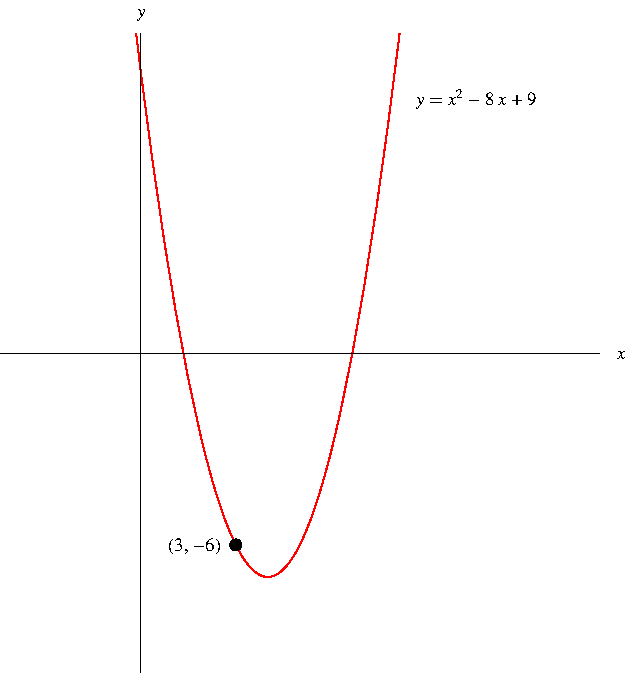
\includegraphics[height=5cm]{derivatives/pictures/03-01-ex5a.pdf}%
}%
\only<6->{%
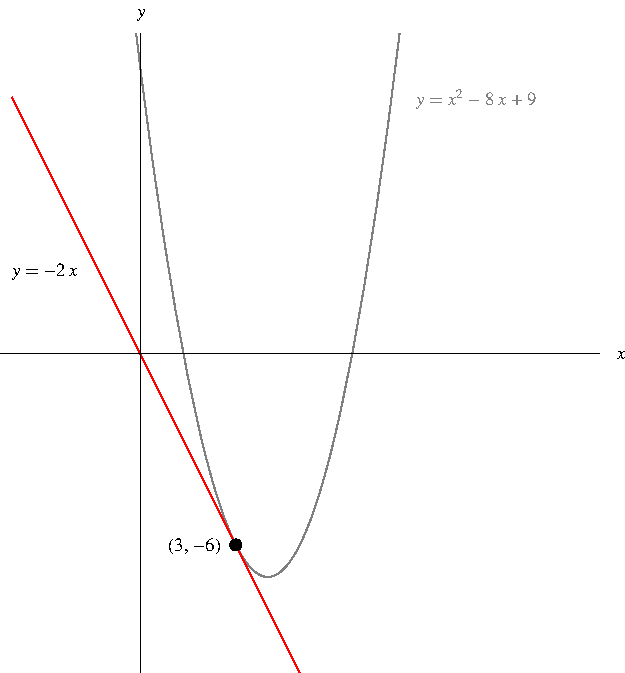
\includegraphics[height=5cm]{derivatives/pictures/03-01-ex5b.pdf}%
}%
\column{.6\textwidth}
\begin{itemize}
\item<2->  The slope of the tangent is the derivative $f'(3)$.
\item<3->  From Example 4, p. 116, $f'(a) = 2a-8$.
\item<4->  Therefore $f'(3) = 2\cdot 3 - 8 = -2$.
\item<5->  Point-slope form: $y - (-6) = -2(x-3)$.
\item<6->  Slope $y$-intercept form: $y = -2x$.
\end{itemize}
\end{columns}
\end{example}
\end{frame}
% end module derivatives-ex5
